%==============================================================================
%  MSDS 498 Capstone --- Exploratory Data Analysis Report
%  NU High School Data Intelligence Platform
%  Write-up of notebooks/EDA_Data_Analysis_Report.ipynb, styled to match
%  MSDS_498_version-wk3.pdf, with the rigor construct grounded in the project's
%  own literature review (Sections 2.2, 2.4, 2.7 of the written report).
%  Compile:  pdflatex MSDS_498_EDA_Report.tex   (run twice for the TOC)
%==============================================================================
\documentclass[12pt,letterpaper]{article}

\usepackage[T1]{fontenc}
\usepackage[utf8]{inputenc}
\usepackage[margin=1in]{geometry}
\usepackage[expansion=false]{microtype}
\usepackage{setspace}
\usepackage{booktabs}
\usepackage{longtable}
\usepackage{array}
\usepackage{ragged2e}
\usepackage{tabularx}
\usepackage{graphicx}
\usepackage{listings}
\usepackage{xcolor}
\usepackage{caption}
\usepackage{textcomp}
\usepackage[hidelinks]{hyperref}
\usepackage{underscore}

%------------------------------------------------------------------ spacing ---
\setstretch{1.15}
\setlength{\parindent}{1.5em}
\captionsetup{font=small,labelfont=bf,skip=6pt}
\captionsetup[longtable]{skip=4pt}

%--------------------------------------------------------------- convenience ---
\newcommand{\ra}{\textrightarrow{}}
\begingroup
\catcode`\/=\active \catcode`\.=\active
\gdef/{\char`\/\allowbreak}
\gdef.{\char`\.\allowbreak}
\endgroup
\newcommand{\code}[1]{{\ttfamily\endlinechar=-1
  \catcode`\/=\active \catcode`\.=\active \scantokens{#1}}}
\tolerance=1200
\emergencystretch=2em
\newcommand{\hd}[1]{\textbf{#1}}

%----------------------------------------------------------------- listings ----
\definecolor{codebg}{gray}{0.965}
\definecolor{codeframe}{gray}{0.80}
\definecolor{kw}{rgb}{0.10,0.10,0.55}
\definecolor{cmt}{rgb}{0.30,0.45,0.30}
\definecolor{str}{rgb}{0.55,0.12,0.12}

\lstdefinestyle{py}{
  language=Python,
  basicstyle=\ttfamily\footnotesize,
  backgroundcolor=\color{codebg},
  frame=single, framesep=6pt, rulecolor=\color{codeframe},
  xleftmargin=8pt, xrightmargin=8pt,
  breaklines=true, breakatwhitespace=false,
  columns=fullflexible, keepspaces=true, showstringspaces=false,
  keywordstyle=\color{kw}\bfseries, commentstyle=\color{cmt}\itshape,
  stringstyle=\color{str}, aboveskip=1em, belowskip=1em,
}
\lstdefinestyle{out}{
  basicstyle=\ttfamily\footnotesize,
  backgroundcolor=\color{codebg!60},
  frame=leftline, framesep=6pt, rulecolor=\color{codeframe},
  xleftmargin=8pt, breaklines=true, columns=fullflexible,
  keepspaces=true, aboveskip=0.6em, belowskip=1em,
}

\hypersetup{pdftitle={MSDS 498 Capstone EDA Report},
  pdfauthor={Max Chalekson, Sheng Hu, Qifan Yang}}

%==============================================================================
\begin{document}

%---------------------------------------------------------------- title page ---
\begin{titlepage}
\centering
\thispagestyle{empty}
\vspace*{1.5in}

{\LARGE\bfseries Exploratory Data Analysis Report\par}
\vspace{0.9em}
{\large The AI-Driven High School Data Intelligence Platform:\\[0.3em]
Coverage, Structure, and the Rigor Construct in Practice\par}

\vspace{1.3in}

{\large Max Chalekson\\ Sheng Hu\\ Qifan Yang\par}

\vspace{0.8in}

{\normalsize Northwestern University\\ Master of Science in Data Science\par}

\vspace{0.7in}

{\normalsize Prepared for Bob Henkins\\ Northwestern Undergraduate Admissions and Enrollment\par}

\vfill
{\normalsize Week 4 Deliverable --- Summer 2026 (2026-07-17)\par}
\end{titlepage}

%------------------------------------------------------------- table of cont ---
\clearpage
\pagenumbering{roman}
\setcounter{tocdepth}{1}
\tableofcontents
\clearpage
\pagenumbering{arabic}

%------------------------------------------------------------------- overview ---
\section*{Overview}
\addcontentsline{toc}{section}{Overview}

This report covers exploratory data analysis on the platform's master dataset,
identifies the data gaps it exposes, assesses the risks those gaps create,
analyzes their impact on the final project, and closes with insights and
recommendations. Every number and chart below is computed live from the project's
actual data (\code{csv_exports/}); nothing here is illustrative or hypothetical.
The analysis draws on \code{benchmarking_v1_2026-07-17.csv} --- the final joined
artifact, covering 53,966 schools nationwide after the rigor-classification,
clustering, and benchmarking passes described in \code{docs/RIGOR_CLASSIFICATION.md},
\code{docs/CLUSTERING.md}, and \code{docs/BENCHMARKING.md} --- together with
\code{clustering_v1_2026-07-17.csv} for the clustering-specific section.

A note on this revision: the rigor sections have been explicitly connected to the
academic-rigor literature the project's written report reviews (Sections 2.2, 2.4,
and 2.7 of \code{MSDS_498_version-wk3}). The intent is to show that the five-tier
rigor scale is not an ad-hoc construct but a deliberate operationalization of a
specific, well-documented body of evidence --- and that this EDA puts several of
that literature's central claims to an empirical test on the project's own data.
Works are cited author--year below; full bibliographic details live in the written
report's Section 2 and bibliography.

The environment used to produce these results is standard: pandas and NumPy for
the tabular work, and Matplotlib with Seaborn for the figures.

\begin{lstlisting}[style=py]
import pandas as pd
import numpy as np
import matplotlib.pyplot as plt
import seaborn as sns

sns.set_theme(style="whitegrid", palette="deep")
plt.rcParams["figure.dpi"] = 110

df = pd.read_csv("../csv_exports/benchmarking_v1_2026-07-17.csv", low_memory=False)
cluster_df = pd.read_csv("../csv_exports/clustering_v1_2026-07-17.csv", low_memory=False)
\end{lstlisting}

\begin{lstlisting}[style=out]
Main dataset:       34,392 rows x 67 columns
Clustering dataset: 34,392 rows x 72 columns
\end{lstlisting}

%==============================================================================
\section{Dataset Overview}
%==============================================================================

The master dataset consolidates ten public data sources --- NCES, Census, CRDC,
College Board, IB, ISBE, CPS, and NAEP --- plus the client's own NU organizational
export, joined primarily on CEEB code. The fully-joined universe
(\code{schools_org_all}) contains 53,966 rows: public schools, private schools, and
org-only rows with no school-side match. The descriptive statistics in this report
use the version restricted to actual public and private high schools with
enrollment at or above 30 --- the ``cleaning freeze'' universe of 34,392 rows
described in \code{docs/TEST_PLAN.md}~\S1. Within that universe the split is 20,620
public schools to 13,772 private, shown in Figure~\ref{fig:sector}.

\begin{lstlisting}[style=py]
print(f"Analysis universe: {len(df):,} schools")
print(df["sector"].value_counts().to_string())

fig, ax = plt.subplots(figsize=(6, 4))
sector_counts = df["sector"].value_counts()
ax.bar(sector_counts.index, sector_counts.values, color=["#4C72B0", "#DD8452"])
ax.set_ylabel("Number of schools")
ax.set_title("Schools by Sector (public vs. private)")
\end{lstlisting}

\begin{figure}[h]
\centering
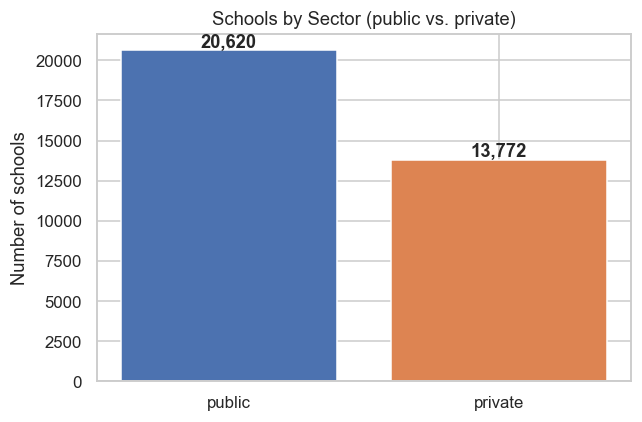
\includegraphics[width=0.6\linewidth]{fig/cell3_1.png}
\caption{Analysis universe by sector: 20,620 public and 13,772 private high schools
(34,392 total).}
\label{fig:sector}
\end{figure}

%==============================================================================
\section{Descriptive Statistics}
%==============================================================================

Table~\ref{tab:desc} summarizes the core numeric features used across the rigor
classification, the funding overlay, and the benchmarking component. Two things are
already visible before any modeling: the features carry very different amounts of
missingness (from 37\% to 68\%), and the ones most central to the rigor construct
--- AP participation and SAT --- are among the least complete, a point Sections 3
and 5 return to.

\begin{table}[h]
\centering
\caption{Descriptive statistics for the core numeric features (34,392-school
universe). ``Miss.\%'' is the share of the universe with a null value.}
\label{tab:desc}
{\footnotesize\setlength{\tabcolsep}{3pt}
\begin{tabular}{@{}>{\RaggedRight\arraybackslash}p{2.7cm} r r r r r r r r r@{}}
\toprule
\hd{Feature} & \hd{Count} & \hd{Mean} & \hd{Std} & \hd{Min} & \hd{25\%} &
\hd{50\%} & \hd{75\%} & \hd{Max} & \hd{Miss.\%} \\
\midrule
\code{grad_rate_2021}         & 17,420 & 84.55  & 17.77  & 0.50    & 82.00    & 91.00    & 95.00    & 99.50     & 49.35 \\
\code{frl_rate}               & 17,230 & 56.52  & 26.19  & 0.12    & 36.02    & 54.29    & 79.07    & 173.77    & 49.90 \\
\code{child_poverty_saipe}    & 20,923 & 15.56  & 7.00   & 2.60    & 10.50    & 14.80    & 19.20    & 60.70     & 39.16 \\
\code{ap_participation}       & 12,260 & 0.19   & 0.15   & 0.00    & 0.08     & 0.16     & 0.26     & 0.78      & 64.35 \\
\code{testtaker_rate}         & 18,804 & 0.20   & 0.15   & 0.00    & 0.07     & 0.20     & 0.28     & 0.71      & 45.32 \\
\code{sat_score_nu}           & 11,098 & 1148.9 & 65.17  & 910.0   & 1110.0   & 1150.0   & 1180.0   & 1440.0    & 67.73 \\
\code{per_resident_child_funding} & 14,340 & 16{,}337 & 6{,}291 & 7{,}842 & 11{,}995 & 14{,}845 & 18{,}920 & 41{,}848 & 58.30 \\
\code{enrollment_9_12}        & 21,638 & 703.4  & 735.85 & 30.0    & 170.0    & 409.0    & 1{,}034  & 14{,}517  & 37.08 \\
\bottomrule
\end{tabular}}
\end{table}

\noindent The \code{frl_rate} maximum of 173.77 is itself a data-quality signal ---
a free/reduced-lunch ``rate'' above 100\% reflects a known denominator mismatch in
the source (enrolled-count versus eligibility-count), documented in
\code{docs/DATA_DICTIONARY.md} --- and is the kind of artifact the coverage and
distribution sections below are designed to surface rather than average away.

%==============================================================================
\section{Data Coverage (Missingness) Analysis}
%==============================================================================

Coverage below 100\% is not inherently a problem --- some fields are legitimately
source-specific, such as the Illinois-only ISBE fields --- but it is exactly what
determines which downstream analyses are trustworthy at what scale, and it is the
foundation for the data-gaps discussion in Section~\ref{sec:gaps}.
Figure~\ref{fig:coverage} ranks the platform's key features by the share of the
universe for which each is populated.

\begin{lstlisting}[style=py]
coverage = pd.Series({label: df[col].notna().mean() * 100
                      for col, label in coverage_cols.items()}).sort_values()
colors = ["#C44E52" if v < 40 else "#DD8452" if v < 70 else "#55A868"
          for v in coverage.values]
ax.barh(coverage.index, coverage.values, color=colors)
\end{lstlisting}

\begin{figure}[h]
\centering
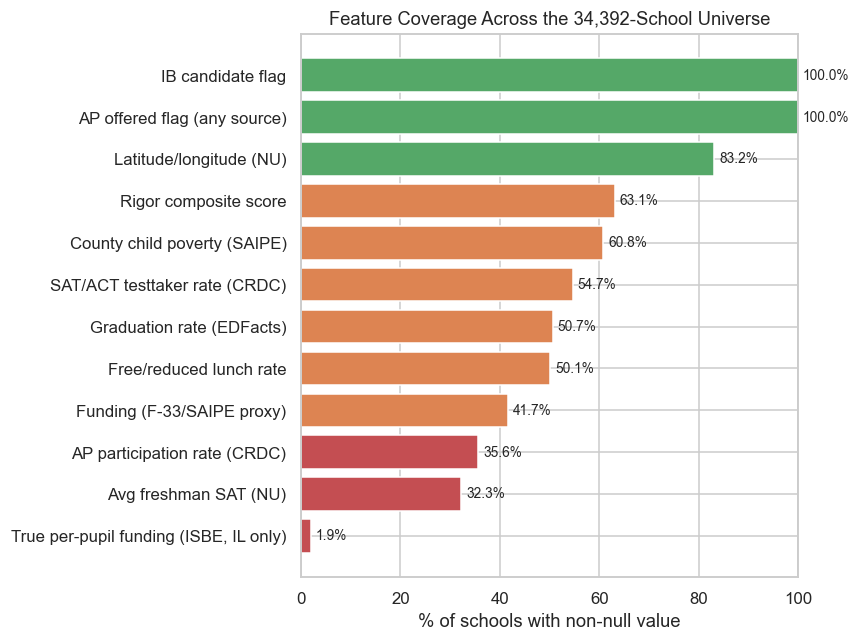
\includegraphics[width=0.78\linewidth]{fig/cell7_2.png}
\caption{Feature coverage across the 34,392-school universe. Red marks features
populated for under 40\% of schools, orange 40--70\%, green above 70\%.}
\label{fig:coverage}
\end{figure}

\noindent The pattern that matters most is not any single bar but where the
rigor-relevant signals fall: the AP and test-participation fields that feed the
rigor tier sit in the middle band, and the rigor composite itself is populated for
under two-thirds of the universe. Section~\ref{sec:private} shows that this missing
third is not missing at random.

%==============================================================================
\section{Data Distributions}
%==============================================================================

Figure~\ref{fig:dist} shows the distributions of the key features feeding the rigor
classification and the funding overlay. The AP-participation and testtaker-rate
distributions are right-skewed and floored at zero, consistent with the
offering-count literature discussed in Section~\ref{sec:rigor}: most schools cluster
at low participation, with a thin tail of high-intensity schools. SAT is
approximately normal but narrow (the bulk between 1,100 and 1,200), and the
enrollment distribution is long-tailed enough that it is clipped at 3,000 for
display.

\begin{lstlisting}[style=py]
fig, axes = plt.subplots(2, 3, figsize=(15, 8))
sns.histplot(df["sat_score_nu"].dropna(), bins=30, ax=axes[0, 0])
sns.histplot(df["ap_participation"].dropna(), bins=30, ax=axes[0, 1])
sns.histplot(df["per_resident_child_funding_state_local"].dropna(), bins=30, ax=axes[0, 2])
sns.histplot(df["child_poverty_saipe"].dropna(), bins=30, ax=axes[1, 0])
sns.histplot(df["grad_rate_2021"].dropna(), bins=30, ax=axes[1, 1])
sns.histplot(df["enrollment_9_12"].dropna().clip(upper=3000), bins=30, ax=axes[1, 2])
\end{lstlisting}

\begin{figure}[h]
\centering
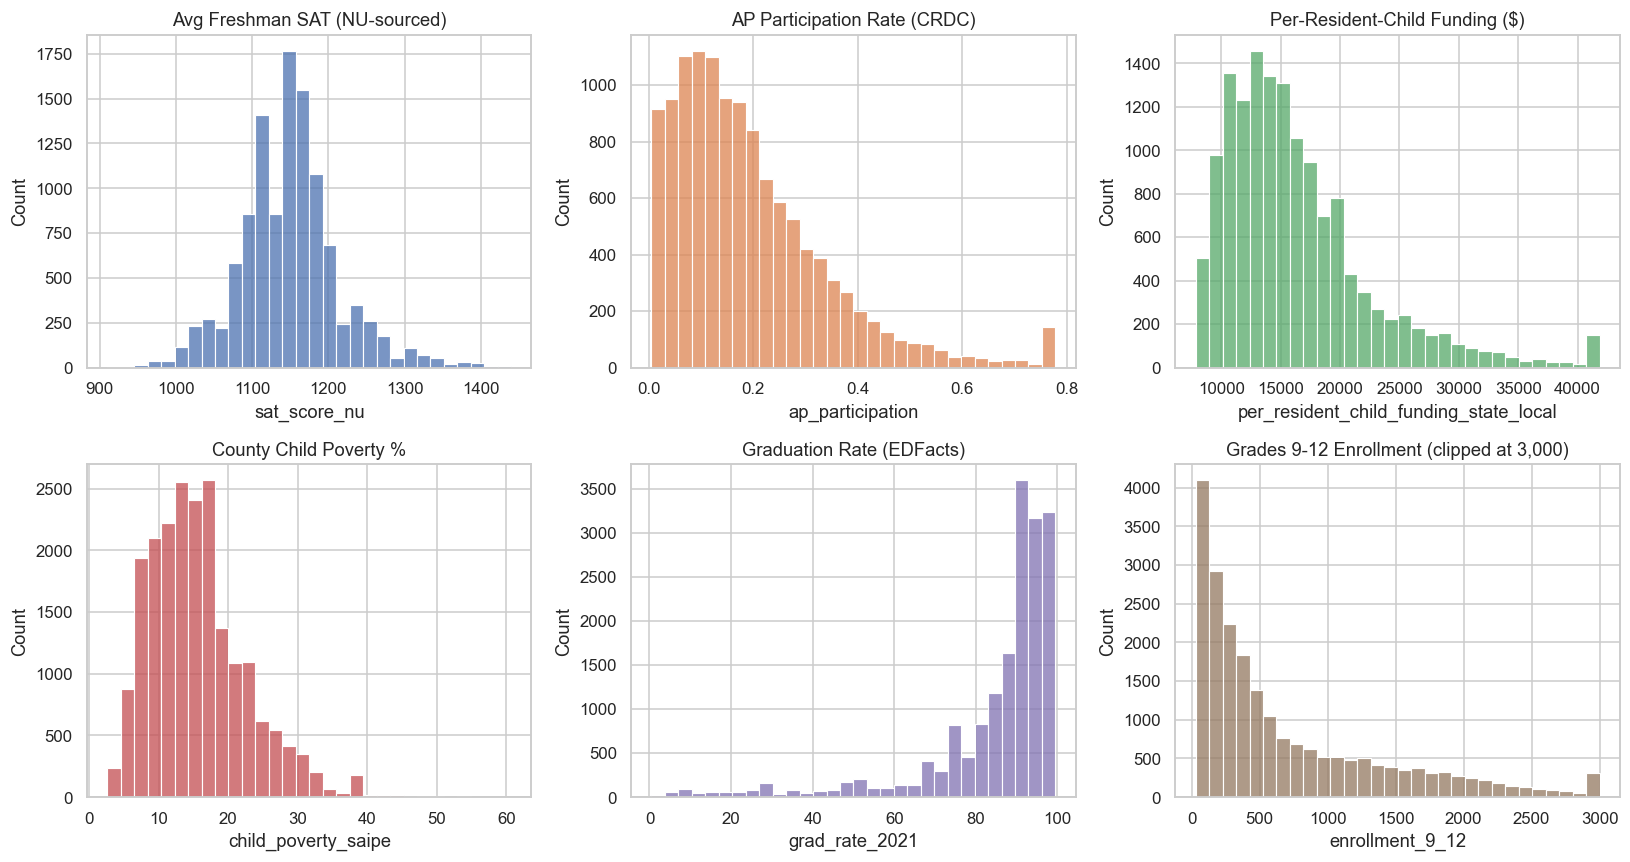
\includegraphics[width=\linewidth]{fig/cell9_3.png}
\caption{Distributions of the six core features feeding the rigor classification and
funding overlay.}
\label{fig:dist}
\end{figure}

%==============================================================================
\section{Public vs.\ Private: The Real Structural Split}\label{sec:private}
%==============================================================================

The single most consequential pattern in this dataset is that public and private
schools have fundamentally different data \emph{availability}, not merely different
values. CRDC --- the richest federal source, carrying AP participation, dual
enrollment, and testtaker rates --- is a public-school-only collection by federal
design; private schools depend entirely on what the client's own NU export happens
to carry. Table~\ref{tab:sectorcov} and Figure~\ref{fig:sectorcov} make the gap
stark: on every CRDC- and EDFacts-sourced feature, private-school coverage is
effectively zero, while the only field with full private-school coverage is the NU
export flag.

\begin{table}[h]
\centering
\caption{Coverage by sector. CRDC- and EDFacts-sourced features are structurally
absent for private schools.}
\label{tab:sectorcov}
{\small
\begin{tabular}{@{}l r r@{}}
\toprule
\hd{Feature} & \hd{Public \%} & \hd{Private \%} \\
\midrule
AP participation (CRDC)        & 59.5  & 0.0 \\
SAT/ACT testtaker rate (CRDC)  & 91.2  & 0.0 \\
Grad rate (EDFacts)            & 84.5  & 0.0 \\
Funding (F-33 proxy)           & 69.5  & 0.0 \\
Has any NU org data            & 100.0 & 100.0 \\
\bottomrule
\end{tabular}}
\end{table}

\begin{figure}[h]
\centering
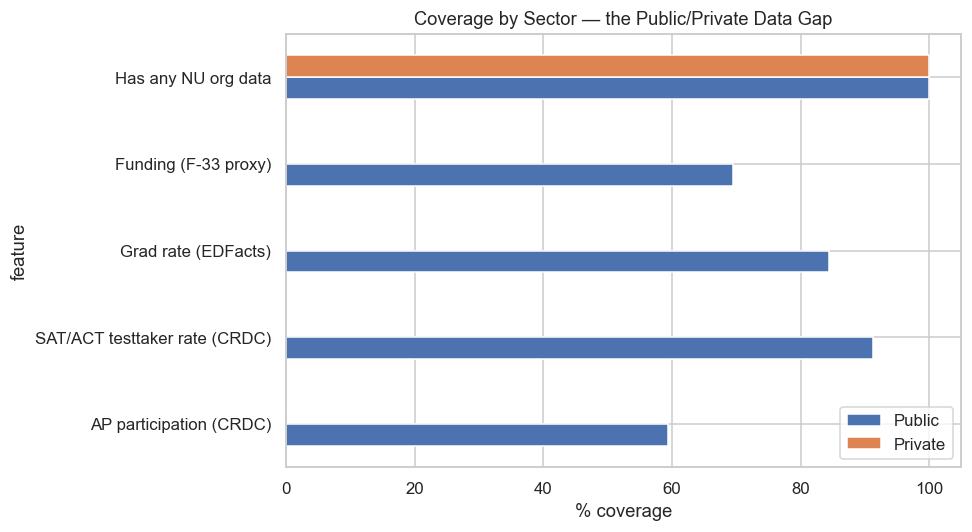
\includegraphics[width=0.82\linewidth]{fig/cell11_4.png}
\caption{Coverage by sector --- the public/private data gap. Every federal source
is public-only; private schools rely entirely on the NU export.}
\label{fig:sectorcov}
\end{figure}

\noindent This is not fixable by better matching: the data simply does not exist for
private schools at the federal level. Its consequence for the rigor construct is
direct and is taken up in Section~\ref{sec:rigor} --- any rigor tier assigned to a
private school rests on a thinner, less-verified foundation than the same tier
assigned to a public one.

%==============================================================================
\section{Correlation Analysis}
%==============================================================================

Figure~\ref{fig:corr} shows the correlations among the academic, funding, and
poverty features that feed the rigor and funding components --- the same
collinearity that \code{docs/CLUSTERING.md}~\S4.3 quantifies via PCA, shown here as
a heatmap for direct inspection. The academic-opportunity features move together,
and both move with funding and (inversely) with poverty. That structure is exactly
what the composite-indicator literature warns about (Section~\ref{sec:rigor}):
when the inputs to a composite are intercorrelated, the composite's nominal weights
diverge from its effective weights, and an offering-based rigor score risks
carrying the socioeconomic signal of its inputs rather than standing apart from it.

\begin{lstlisting}[style=py]
corr_cols = ["ap_participation", "dual_enrollment_rate", "testtaker_rate",
             "grad_rate_2021", "per_resident_child_funding_state_local",
             "child_poverty_saipe", "latitude", "longitude"]
sns.heatmap(df[corr_cols].corr(), annot=True, fmt=".2f", cmap="RdBu_r",
            center=0, vmin=-1, vmax=1)
\end{lstlisting}

\begin{figure}[h]
\centering
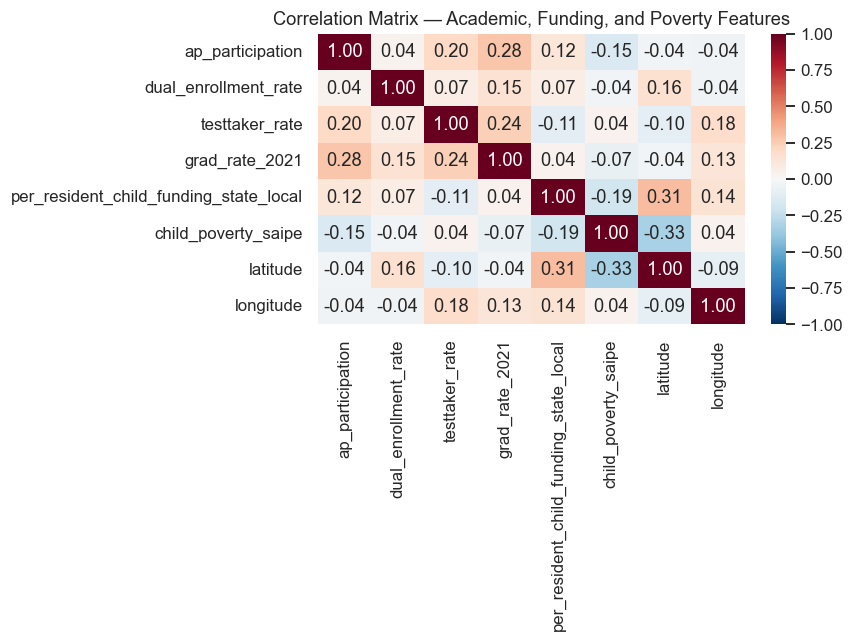
\includegraphics[width=0.72\linewidth]{fig/cell13_5.png}
\caption{Correlation matrix among academic, funding, and poverty features.}
\label{fig:corr}
\end{figure}

%==============================================================================
\section{Rigor Classification Summary}\label{sec:rigor}
%==============================================================================

The rigor tier is a five-level composite built from AP, CRDC-coursework, and
test-participation components; the full methodology, including the nominal-versus-
effective weights and the sensitivity analysis, is in
\code{docs/RIGOR_CLASSIFICATION.md}. Figure~\ref{fig:rigor} shows the tier
distribution, and the composite is populated for 21,706 of the 34,392 schools
(63.1\%).

\begin{lstlisting}[style=py]
tier_order = ["Below Average", "Average", "Demanding",
              "Very Demanding", "Most Demanding"]
tier_counts = df["rigor_tier_label"].value_counts().reindex(tier_order)
ax.bar(tier_counts.index, tier_counts.values, color=sns.color_palette("viridis", 5))
print(f"Scored: {df['rigor_score'].notna().sum():,} / {len(df):,} "
      f"({100*df['rigor_score'].notna().mean():.1f}%)")
\end{lstlisting}

\begin{figure}[h]
\centering
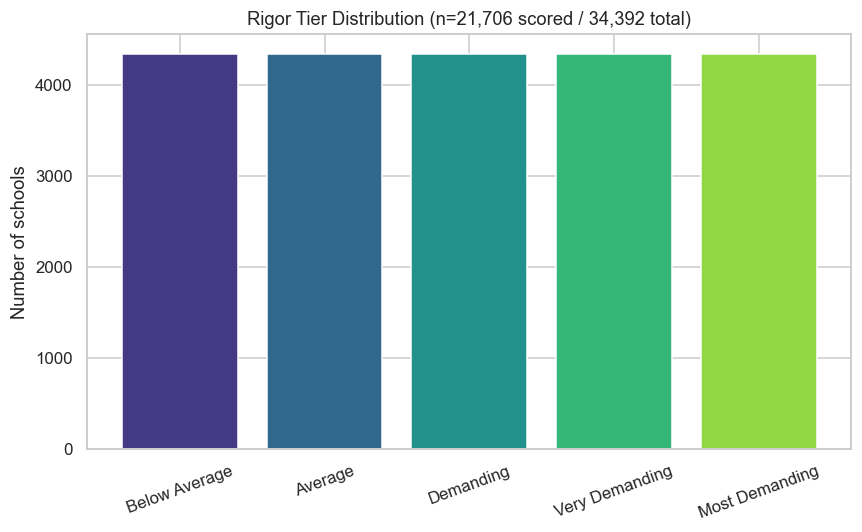
\includegraphics[width=0.78\linewidth]{fig/cell15_6.png}
\caption{Rigor tier distribution across the 21,706 scored schools.}
\label{fig:rigor}
\end{figure}

\begin{lstlisting}[style=out]
Scored: 21,706 / 34,392 (63.1%)
\end{lstlisting}

\subsection*{Grounding in the rigor literature}

The five-tier scale is a deliberate operationalization of the construct the
project's written report adopts (Section 2.2), not an ad-hoc index. Adelman's two
U.S.\ Department of Education longitudinal studies, \emph{Answers in the Tool Box}
(Adelman, 1999) and \emph{The Toolbox Revisited} (Adelman, 2006), established
curriculum intensity --- not test scores or GPA --- as the single strongest
predictor of bachelor's-degree completion, accounting for roughly 43\% of variance
in the earlier study; that finding is what justifies building a rigor measure from
course-offering data at all. The same literature, however, bounds what such a
measure can claim. Geiser and Santelices (2004) found that AP and honors
course-\emph{taking} carried little predictive validity for college outcomes once
other factors were controlled, while AP \emph{exam performance} did, and the tier
here is built almost entirely from availability and participation data --- CRDC AP
counts, IB flags with no U.S.\ exam scores, and state AP aggregates --- rather than
exam outcomes. The tier therefore measures \emph{opportunity structure}, what a
school offers, rather than demonstrated academic outcome, and is most honestly read
as a ``most opportunity-rich'' scale rather than a ``most demanding'' one.

The coverage numbers reinforce that reading. The signal exists for only 63.1\% of
the universe, and Section~\ref{sec:private} showed that the missing 36.9\% is
concentrated among private schools, not spread at random. Two further strands of the
literature explain why the correlation and poverty checks in this report are not
optional. Kolluri (2018) documents that low-income students enroll in AP, where it
is offered, at under a third the rate of higher-income peers, and that nearly all
AP-effectiveness studies are correlational; the U.S.\ Government Accountability
Office (2018) found directly that high-poverty and smaller schools offer fewer
college-preparatory courses. A rigor tier built from offering counts will therefore
tend to proxy school size and affluence, which means the funding and poverty overlay
is not guaranteed to be an independent enrichment layer --- it may be collinear with
the rigor target itself, exactly the collinearity visible in Section~6's heatmap.
Whether this project's tier actually inherited that confound is an empirical
question, and Section~\ref{sec:bench} answers it.

%==============================================================================
\section{Clustering Summary}
%==============================================================================

Figure~\ref{fig:cluster} plots the K-means clusters ($k=4$, selected via the gap
statistic) on the first two principal components. The full methodology is in
\code{docs/CLUSTERING.md}, including the honest finding that cluster separation is
weak (best silhouette score 0.205, below the conventional 0.25 threshold), shown
visually here as overlapping rather than tightly separated point clouds. Complete-
case coverage across all eight clustering features (location, academic, funding, and
poverty) exists for only 5,797 schools --- 16.9\% of the universe --- which is
itself a finding: the clustering speaks for a minority of well-covered schools, not
the whole platform.

\begin{lstlisting}[style=py]
plot_df = cluster_df.dropna(subset=["pca_component_1", "pca_component_2",
                                    "cluster_kmeans"])
ax.scatter(plot_df["pca_component_1"], plot_df["pca_component_2"],
           c=plot_df["cluster_kmeans"], cmap="Set2", alpha=0.4, s=10)
\end{lstlisting}

\begin{figure}[h]
\centering
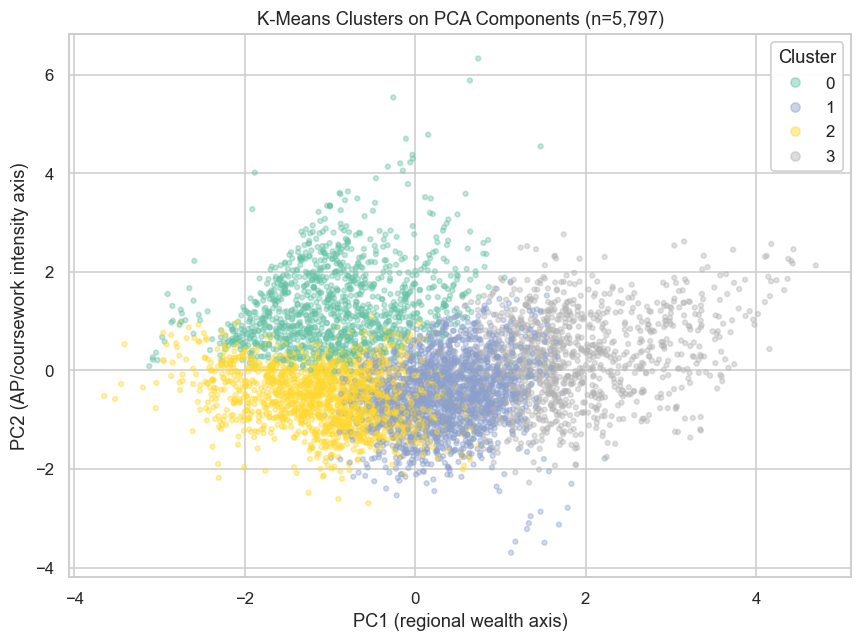
\includegraphics[width=0.72\linewidth]{fig/cell17_7.png}
\caption{K-means clusters on the first two principal components ($n=5{,}797$
complete cases). PC1 reads as a regional-wealth axis, PC2 as AP/coursework
intensity.}
\label{fig:cluster}
\end{figure}

\begin{lstlisting}[style=out]
Complete-case coverage for clustering: 5,797 / 34,392 (16.9%)
\end{lstlisting}

%==============================================================================
\section{Performance Benchmarking Summary}\label{sec:bench}
%==============================================================================

Figure~\ref{fig:bench} shows mean SAT by region and by rigor tier (descriptive only;
the full peer-group methodology and the socioeconomic-reproduction finding are in
\code{docs/BENCHMARKING.md}). The decisive numbers are the two rank correlations
printed beneath it: SAT achievement correlates $-0.385$ with county child poverty,
while the rigor tier correlates only $-0.070$.

\begin{lstlisting}[style=py]
region_sat = df.groupby("us_region")["sat_score_nu"].mean().sort_values(ascending=False)
tier_sat = df.groupby("rigor_tier_label")["sat_score_nu"].mean().reindex(tier_order)
print(f"spearman(SAT, poverty)        = "
      f"{df['sat_score_nu'].corr(df['child_poverty_saipe'], method='spearman'):.3f}")
print(f"spearman(rigor tier, poverty) = "
      f"{df['rigor_tier_num'].corr(df['child_poverty_saipe'], method='spearman'):.3f}")
\end{lstlisting}

\begin{figure}[h]
\centering
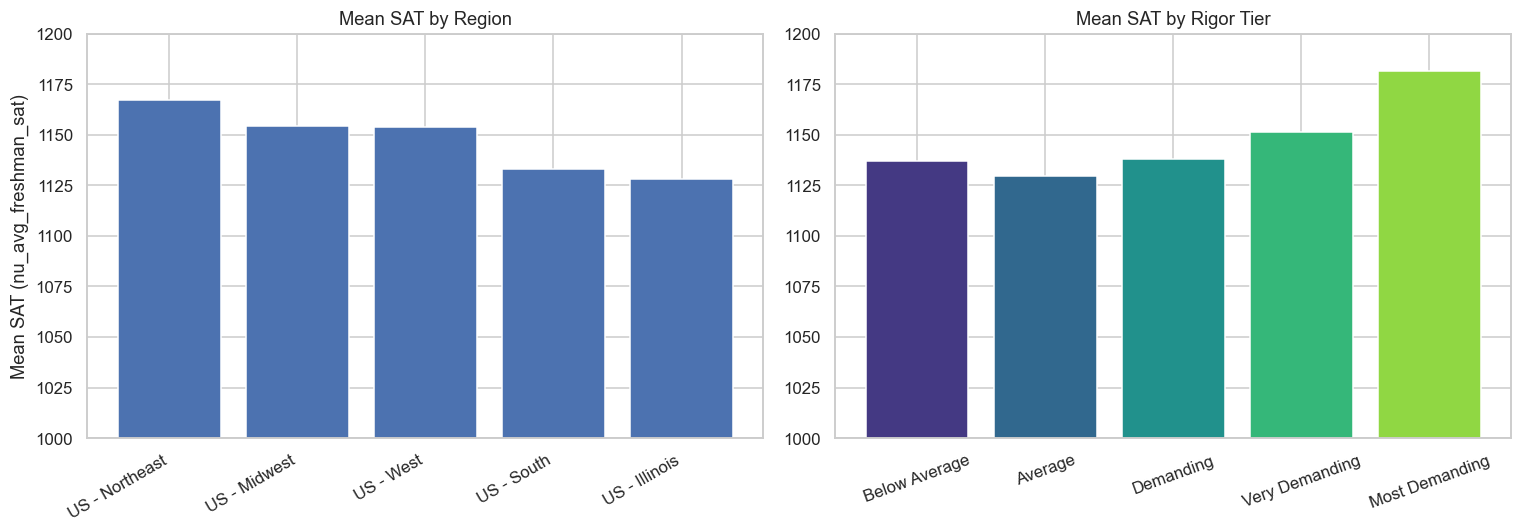
\includegraphics[width=\linewidth]{fig/cell19_8.png}
\caption{Mean SAT by region (left) and by rigor tier (right).}
\label{fig:bench}
\end{figure}

\begin{lstlisting}[style=out]
spearman(SAT, poverty)        = -0.385
spearman(rigor tier, poverty) = -0.070
\end{lstlisting}

\noindent This is the composite-indicator literature's central warning put to an
empirical test on the project's own data. The Stanford Education Data Archive work
(Jang and Reardon, 2019; Ho, 2020) established that achievement-\emph{level}
indicators are powerfully predicted by socioeconomic composition and therefore
reproduce the socioeconomic ordering of American schools --- which is precisely what
the SAT correlation of $-0.385$ shows here, an outcome-style measure ranking
affluent schools highest and under-resourced schools lowest, the opposite of what
the platform's gap-detection purpose requires. The rigor tier, built from
opportunity structure rather than outcomes, does not reproduce that ordering to
nearly the same degree ($-0.070$). The concern raised in Section~\ref{sec:rigor} ---
that offering counts might smuggle the socioeconomic signal back in --- is thus
tested and found small in this design, consistent with Bastedo et al.\ (2022, 2023),
who show that contextualized, opportunity-oriented measures improve both equity and
predictive accuracy relative to raw scores. The caution that remains is the one
Geiser and Studley (2002) and Bettinger et al.\ (2013) name: an undisaggregated SAT
or ACT benchmark averages sub-scores of very different predictive validity and very
different income sensitivity, so the benchmarking layer should report section-level
aggregates wherever the data permit.

%==============================================================================
\section{Identification of Data Gaps}\label{sec:gaps}
%==============================================================================

Every gap below is drawn directly from the coverage numbers computed above, together
with findings documented in \code{docs/DATA_DICTIONARY.md},
\code{docs/EDA_features_joined.md}, and \code{docs/BOB_BRIEFING.md} during the
project's development.

The first and most consequential is the \textbf{structural gap for private schools}.
CRDC --- the richest source, carrying AP participation, dual enrollment, and
testtaker rates --- is public-school-only by federal design.
Section~\ref{sec:private} shows this starkly: private schools have near-zero CRDC
coverage regardless of school quality. This is not fixable by better matching,
because the data simply does not exist for private schools at the federal level;
only the client's NU export fills it, and only where NU has data.

The second is a set of \textbf{vintage and freshness gaps}. Most \code{nu_*} fields
(56 of them) carry no confirmed per-variable measurement date, only the export
file's timestamp. CRDC's vintage is confirmed (SY2021-22) for the CRDC file itself,
but that file arrives bundled inside a teammate's gitignored export, so its
freshness cannot be independently re-verified from this repo's own history (see the
2026-07-17 update in \code{docs/DATA_DICTIONARY.md}).

The third is \textbf{coverage, quantified}, from Section~3: rigor-classifier signal
exists for only 63.1\% of the universe; complete data across all eight clustering
features exists for only 16.9\%; SAT coverage is 32.3\%; and ACT coverage is 1.2\%
nationally, effectively unusable outside Illinois.

The fourth is \textbf{identifier and linkage gaps}. The \code{custom_id} field in
the client's org export matches no federal ID system and is not unique, making it
unusable as a join key. Investigating it surfaced a separate and more serious
finding: at least 62 confirmed (644 suspected) CEEB codes show a digit-shift
corruption pattern, meaning some schools' primary join key may itself be wrong.

The fifth is the \textbf{true per-pupil funding gap}. Census F-33 has no
enrollment or membership field, and no verified district-level enrollment source is
loaded, so the national funding feature is a population-based proxy (SAIPE
school-age residents) rather than true per-pupil expenditure.

%==============================================================================
\section{Assessment of Associated Risks}
%==============================================================================

Table~\ref{tab:risk} records the risks these gaps create, each with its likelihood,
severity, and the specific evidence behind it. None is speculative; every entry
points to a quantified finding in the project's own record.

{\small
\begin{longtable}{@{}>{\RaggedRight\arraybackslash}p{0.28\textwidth}
                     >{\RaggedRight\arraybackslash}p{0.15\textwidth}
                     >{\RaggedRight\arraybackslash}p{0.10\textwidth}
                     >{\RaggedRight\arraybackslash}p{0.37\textwidth}@{}}
\caption{Risk register for the platform's data gaps.}\label{tab:risk}\\
\toprule
\hd{Risk} & \hd{Likelihood} & \hd{Severity} & \hd{Evidence} \\
\midrule
\endfirsthead
\multicolumn{4}{@{}l}{\itshape Table \ref{tab:risk} continued}\\[2pt]
\toprule
\hd{Risk} & \hd{Likelihood} & \hd{Severity} & \hd{Evidence} \\
\midrule
\endhead
\midrule
\multicolumn{4}{r@{}}{\itshape continued on next page}\\
\endfoot
\bottomrule
\endlastfoot

CRDC access loss changes rigor tiers substantially &
Confirmed, not hypothetical & High &
52.5\% of CRDC-covered schools change rigor tier if the CRDC signal is removed
(\code{docs/RIGOR_CLASSIFICATION.md}) --- quantified, not estimated. \\
\addlinespace

Private schools systematically under-represented in rigor/funding features &
Certain (structural) & High &
Section~\ref{sec:private}; a platform meant to serve \emph{all} applicants has a
built-in blind spot for $\sim$13,900 private high schools. \\
\addlinespace

Rigor tier could reproduce socioeconomic ordering, undermining the core value
proposition & Checked, found low & Low (currently) &
Rigor-tier/poverty correlation is only $-0.070$, versus $-0.385$ for raw SAT --- the
risk is real for outcome-style measures but empirically low for this
opportunity-structure design. \\
\addlinespace

CEEB corruption causes silent school mis-attribution &
Confirmed for 62+ codes & Medium &
A corrupted CEEB could attach a school's data to the wrong record, or fail to match
at all, without any error being raised. \\
\addlinespace

Funding proxy misrepresents true per-pupil spending &
Certain (by construction) & Medium &
Population $\div$ revenue is not the same denominator as enrolled students; districts
with unusual population-to-enrollment ratios are most affected. \\
\addlinespace

Weak natural cluster structure over-interpreted as meaningful school ``types'' &
Confirmed & Medium &
Silhouette score 0.205 (below the conventional 0.25 threshold) --- any narrative
built on hard cluster boundaries would overstate what the data support. \\
\addlinespace

Reproducibility gap: a new team member or grader cannot rebuild the full pipeline &
Confirmed, mitigated & Low (after mitigation) &
Fixed 2026-07-17 --- the raw data ($\sim$2.6~GB) is documented via a shared Drive
link rather than left unwritten. \\
\end{longtable}
}

%==============================================================================
\section{Impact Analysis and Mitigation Strategies}
%==============================================================================

\noindent\textbf{CRDC dependency (High).} If the Office for Civil Rights, CRDC's
steward, changes access terms --- a real possibility already flagged in the
project's literature review --- roughly half of currently-tiered schools would need
re-scoring, and their tier could change. The mitigation already in place is that the
rigor classifier logs which components were available per school
(\code{rigor_components_available}), so a future CRDC loss is detectable and
auditable rather than silent; the recommendation is to monitor CRDC's release
cadence and maintain the NU-only fallback scenario, which is already built and
tested.

\noindent\textbf{Private-school gap (High).} Any rigor-tier or benchmarking claim
about private schools rests on a thinner, less-verified foundation than the same
claim about public schools --- a direct threat to the platform's stated goal of
being \emph{more} equitable than Landscape, not merely a replacement for it. The
sector split is already surfaced everywhere rather than hidden inside an aggregate
``all schools'' number, and this report documents it explicitly; the recommendation
is to state the limitation plainly in any client-facing deliverable that includes
private schools, and to treat public and private as two separate populations for any
statistical claim rather than one blended one.

\noindent\textbf{CEEB corruption (Medium).} Up to 644 schools (62 confirmed) may
have data misattributed via the join key, undermining trust in any number derived
from a match. The corruption is flagged via \code{ceeb_suspected_padding_shift}
rather than silently corrected, since there is no reliable way to determine which
side of a pair is right; the recommendation is to raise it with whoever owns the
source export, since this is an upstream data-entry issue rather than something
fixable downstream.

\noindent\textbf{Funding proxy (Medium).} Any per-pupil funding comparison is only
as good as the population-based proxy, which could be off in either direction for
specific districts. It is labeled distinctly from the true per-pupil Illinois figure
via \code{funding_source}, so the two are never silently averaged; the recommendation
is to source a true district-enrollment file (NCES CCD membership) to replace the
proxy --- not blocked on anyone, simply not yet done.

\noindent\textbf{Weak cluster structure (Medium).} There is a risk of overstating
findings in the final presentation or paper if cluster assignments are treated as
ground truth. The weak silhouette score is already reported as a finding about the
data rather than hidden or re-framed as a modeling failure; the recommendation is
that any cluster-based narrative in the final paper carry the silhouette score
alongside it.

%==============================================================================
\section{Insights and Recommendations}
%==============================================================================

\noindent\textbf{Insight 1 --- opportunity-structure measures beat outcome measures
on equity, and now there is data to prove it, not just cite it.} SAT achievement
correlates $-0.385$ with poverty; the rigor tier, built from AP, coursework, and
test-participation \emph{offerings} rather than scores, correlates only $-0.070$.
This is the central claim of the written report's literature review (Sections 2.2
and 2.4 --- Adelman, 1999, 2006; Jang and Reardon, 2019; Ho, 2020) demonstrated on
the project's own data rather than merely cited. It should lead the final paper's
Discussion, since it is a genuinely novel empirical contribution, not a restatement
of prior work.

\noindent\textbf{Insight 2 --- the platform's biggest limitation is not data
quality, it is data existence.} Most gaps identified here --- private-school CRDC
absence, ACT sparsity, vintage uncertainty --- are not fixable by better joins or
cleaner code, because the underlying federal and commercial data does not exist at
the needed grain. This should be framed honestly in the final paper as a structural
finding about the U.S.\ education-data landscape, consistent with the Section~2
literature review and with the client's own framing (``there's a lot of gaps in the
higher-ed industry'' --- Bob Henkins, 2026-07-14 meeting).

\noindent\textbf{Insight 3 --- the platform is more reliable for public schools than
private, and the paper should say so} rather than presenting one blended accuracy
claim. A sector-split validation section is preferable to a single aggregate metric.

\noindent\textbf{Recommendation.} Prioritize closing the CRDC-dependency and
CEEB-corruption risks before the Week 9 presentation. Both are quantified, both have
a clear owner --- CRDC monitoring for whoever tracks OCR policy, CEEB corruption for
whoever owns the upstream export --- and both currently sit as open items rather than
resolved ones.

%==============================================================================
\section{Conclusion}
%==============================================================================

The dataset underlying this platform is large --- 53,966 schools across ten source
systems --- and, after the fixes made during development (LEAID derivation, the CEEB
fan-out, sector misclassification), internally consistent: the Docker-backed and
CSV-backed pipelines produce identical results, and 57 automated tests pass. But
internal consistency is not completeness. The real constraints on this platform are
structural --- private schools lack CRDC by design --- and are not corrigible by
more engineering. The strongest finding to come out of this EDA is a positive one,
and a literature-grounded one: the rigor tier is meaningfully less socioeconomically
confounded than raw achievement scores, exactly the property the rigor construct was
chosen for and the property the composite-indicator literature warned an
offering-based measure might fail to have. The most important open risk is the
CRDC-dependency finding, since half of currently-tiered schools would shift tier if
that single federal source became unavailable. Both belong prominently in the final
paper, not buried in an appendix.

\subsection*{A note on citations}

The works referenced above --- Adelman (1999, 2006); Geiser and Santelices (2004);
Kolluri (2018); U.S.\ Government Accountability Office (2018); Coca et al.\ (2012);
Bastedo et al.\ (2022, 2023); Jang and Reardon (2019); Ho (2020); Geiser and Studley
(2002); Bettinger et al.\ (2013) --- are the same sources reviewed in Section~2 of
the project's written report (\code{MSDS_498_version-wk3}); full bibliographic
details appear in that document's bibliography and are not duplicated here.

\end{document}
